\documentclass[10pt,xcolor={dvipsnames}]{beamer}
\usetheme[
%%% option passed to the outer theme
%    progressstyle=fixedCircCnt,   % fixedCircCnt, movingCircCnt (moving is deault)
  ]{Feather}

%\definecolor{NavyBlue}{rgb}{0.0, 0.0, 0.5} 
\definecolor{NavyBlue}{rgb}{0.0, 0.47, 0.75} %azul
%\definecolor{NavyBlue}{rgb}{1.0, 0.35, 0.21} %naranja
%\definecolor{NavyBlue}{rgb}{0.8, 0.6, 0.8} %morado
%\definecolor{NavyBlue}{rgb}{0.63, 0.36, 0.94}  
  
% If you want to change the colors of the various elements in the theme, edit and uncomment the following lines

% Change the bar colors:
\setbeamercolor{Feather}{fg=NavyBlue!20,bg=NavyBlue}

% Change the color of the structural elements:
\setbeamercolor{structure}{fg=NavyBlue}

% Change the frame title text color:
\setbeamercolor{frametitle}{fg=black!5}

% Change the normal text colors:
\setbeamercolor{normal text}{fg=black!75,bg=gray!5}

%% Change the block title colors
\setbeamercolor{block title}{use=Feather,bg=Feather.fg, fg=black!90} 


% Change the logo in the upper right circle:
%\renewcommand{\logofile}{example-grid-100x100pt} 
%% This is an image that comes with the LaTeX installation
% Adjust scale of the logo w.r.t. the circle; default is 0.875
% \renewcommand{\logoscale}{0.55}

% Change the background image on the title and final page.
% It stretches to fill the entire frame!
% \renewcommand{\backgroundfile}{example-grid-100x100pt}

%-------------------------------------------------------
% INCLUDE PACKAGES
%-------------------------------------------------------

\usepackage[utf8]{inputenc}
\usepackage[english]{babel}
\usepackage[T1]{fontenc}
% \usepackage{helvet}

%% Load different font packages to use different fonts
%% e.g. using Linux Libertine, Linux Biolinum and Inconsolata
% \usepackage{libertine}
% \usepackage{zi4}

%% e.g. using Venturis ADF Serif and Sans
% \usepackage{venturis}

%-------------------------------------------------------
% DEFFINING AND REDEFINING COMMANDS
%-------------------------------------------------------

% colored hyperlinks
\newcommand{\chref}[2]{
  \href{#1}{{\usebeamercolor[bg]{Feather}#2}}
}

%-------------------------------------------------------
% INFORMATION IN THE TITLE PAGE
%-------------------------------------------------------

\title[Fund Computación] % [] is optional - is placed on the bottom of the sidebar on every slide
{ % is placed on the title page
      \Large{\textbf{Fundamentación en computación}}
}

\subtitle[Clase 1]
{
      \textbf{Sistemas operativos}
}

\author[Julián Calle]
{      Julián Calle \\
      {\ttfamily julian.callem@udea.edu.co}\\[1em]
      Taller 2
}

\institute[UdeA]
{%
\begin{columns}
\begin{column}{3cm}

\includegraphics[scale=0.045]{Feathergraphics/2-2} 
\end{column}
\begin{column}{6cm} 
Instituto de física\\
Facultad de ciencias exactas y naturales \\
Universidad de Antioquia
\end{column} \end{columns}
}

\date{\today}

%-------------------------------------------------------
% THE BODY OF THE PRESENTATION
%-------------------------------------------------------

\begin{document}

%-------------------------------------------------------
% THE TITLEPAGE
%-------------------------------------------------------

{\1
\begin{frame}[plain,noframenumbering]
  \titlepage
\end{frame}}


\begin{frame}{Content}{}
\tableofcontents
\end{frame}


\section{Sistemas operativos}
\begin{frame}
\begin{center}
\Huge{\textcolor{blue}{Sistemas operativos}}
\end{center}
\end{frame}

\begin{frame}
\begin{itemize}
\item<1-3|alert@1> Permite realizar multiples tareas.
\item<2-3|alert@2> Permite administrar e intalar los programas que necesitas.
\item<3-3|alert@3> Permite el uso de Drivers.
\item<4-|alert@4> Lenguaje de maquina
\item<5-|alert@5> 1954: IBM-704
\item<6-|alert@6> 1964: Creación de Unics, luego paso a Unix.
\item<7-|alert@7> 70’s: Aparecen las computadoras personales con sus SO
\item<8-|alert@8> 1980: Windows crea xenix SO para sus computadoras
\item<9-|alert@9> 1981: MS Dos de windows aparece.
\item<10-|alert@10> 90’s: Aparece GNU/Linux.
\end{itemize}
\end{frame}

\begin{frame}
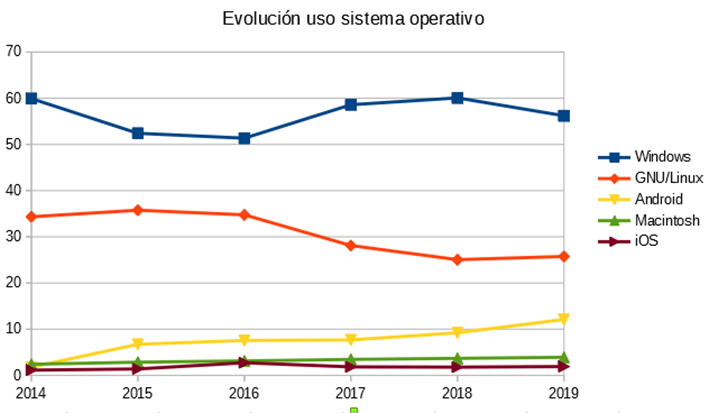
\includegraphics[scale=0.4]{Figures/evolucionSO}
\end{frame}

\subsection{Windows}
\begin{frame}
\begin{center}
\Huge{\textcolor{blue}{Windows}} \\ \vspace{0.5cm}

\includegraphics[scale=0.5]{Figures/windows}
\end{center}
\end{frame}

\begin{frame}{Fundadores}
\begin{center}
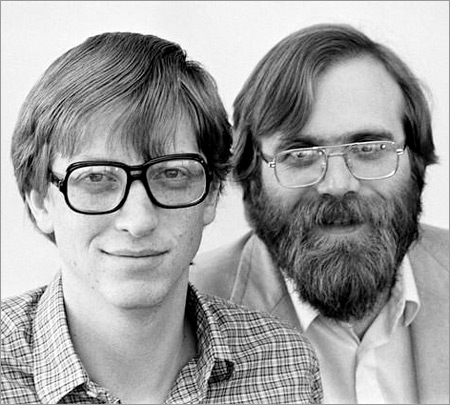
\includegraphics[scale=0.45]{Figures/Bill-Gates-y-Paul-Allen} \\
Bill Gates y Paul Allen
\end{center}
\end{frame}

\begin{frame}{Windows}
\begin{center}
\only<1>{\Large{1985} \\ 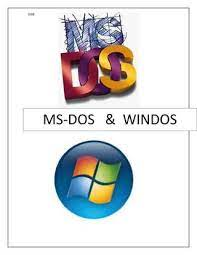
\includegraphics[scale=0.5]{Figures/MSDOS}}
\only<2->{
\includegraphics[scale=0.2]{Figures/windows}}
\begin{itemize}
\item<3-|alert@3> Tiene más variedad de programas.
\item<4-|alert@4> Tiene más soporte.
\item<5-|alert@5> Linea de comandos no tan útil, se utiliza más la interfaz grafica.
\item<6-|alert@6> Hay que configurar el SO para programar.
\item<7-|alert@7> Es posible tener la misma calidad (excepto MacOS).
\item<8-|alert@8> Ahora se puede usar la consola de Linux en Windows.
\end{itemize}
\end{center}
\end{frame}

\subsection{Linux}
\begin{frame}
\begin{center}
\Huge{\textcolor{blue}{Linux}} \\ \vspace{0.5cm}

\includegraphics[scale=0.15]{Figures/LINUX}
\end{center}
\end{frame}

\begin{frame}{Fundadores}
\begin{center}
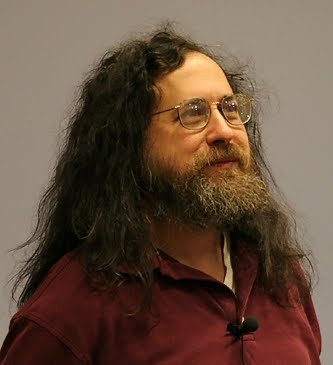
\includegraphics[scale=0.3]{Figures/Richard_Stallman}
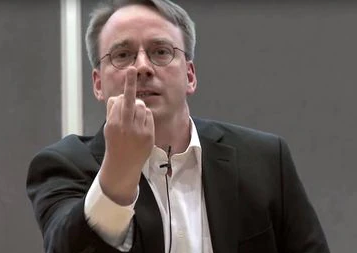
\includegraphics[scale=0.58]{Figures/Linus} \\
Richard Stallman y Linus Torvalds
\end{center}
\end{frame}

\begin{frame}{Linux}
\only<1>{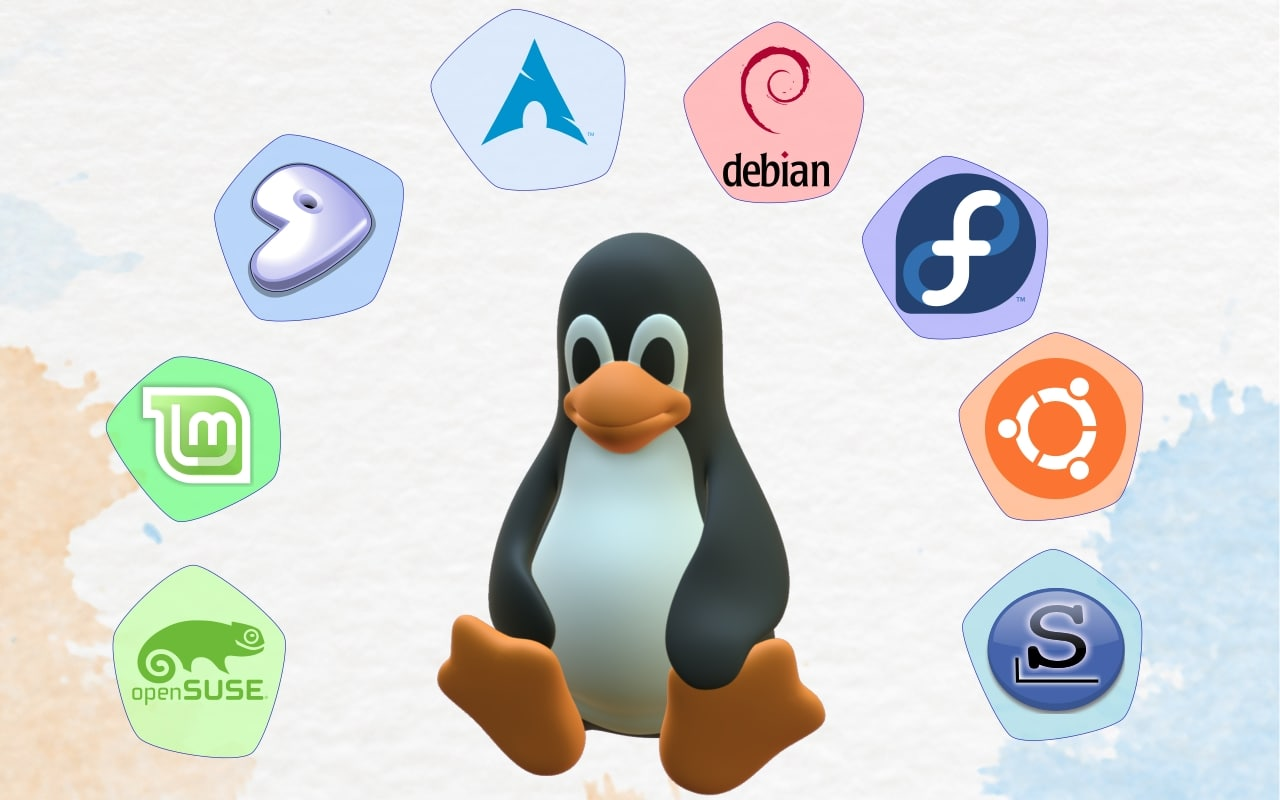
\includegraphics[scale=0.22]{Figures/linuxDist}}
\only<2>{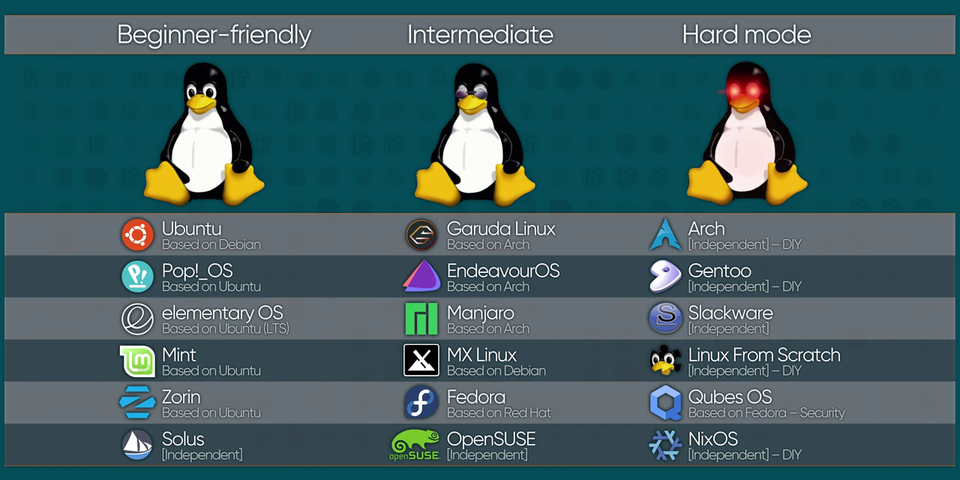
\includegraphics[scale=0.45]{Figures/LinuxDif}}
\end{frame}

\begin{frame}{Linux}
\begin{center}
\only<1>{\Large{1993} \\ 
\includegraphics[scale=0.4]{Figures/gnulinux}}
\only<2->{
\includegraphics[scale=0.05]{Figures/LINUX}}
\begin{itemize}
\item<3-|alert@3> Linux y seguridad: Evita virus y malware.
\item<4-|alert@4> Nunca se tiene seguridad al 100\%, siempre puede ser vulnerado.
\item<5-|alert@5> Fuciones de root.
\item<6-|alert@6> Es un sistema Open source.
\item<7-|alert@7> Optimización, permite usarse en maquinas viejas y nuevas. 
\item<8-|alert@8> Líneas de comando de bash (bourne again shell).
\item<9-|alert@9> Flexibles, escalables y personalizable.
\item<10-|alert@10> Soporte, comunidad y documentación: Comunidad de gente con tus mismo problemas.
\item<11-|alert@11> Es gratis, sus herramientas son gratis y open source. Podes hacer lo que quieras con ellas.
\item<12-|alert@12> SO más usado en servidores.
\item<13-|alert@13> Software alternativo: open office, entre otros.
\end{itemize}
\end{center}
\end{frame}


\subsection{Mac OS}
\begin{frame}
\begin{center}
\Huge{\textcolor{blue}{Mac OS}} \\ \vspace{0.5cm}

\includegraphics[scale=0.35]{Figures/MCOs}
\end{center}
\end{frame}

\begin{frame}{Fundadores}
\begin{center}
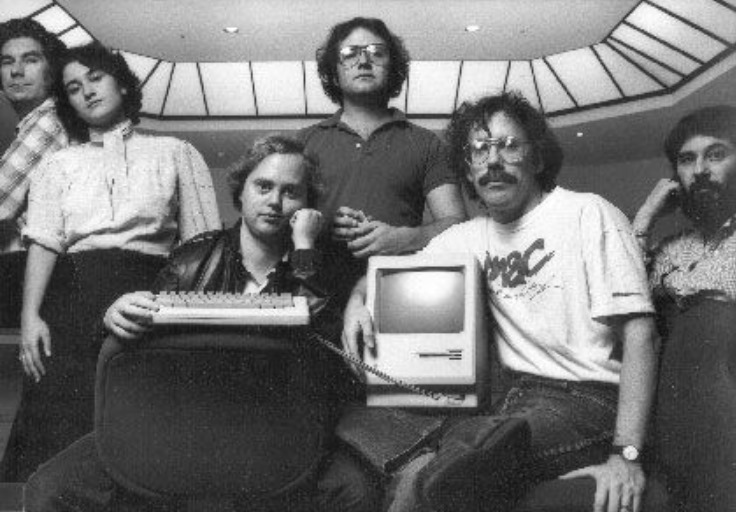
\includegraphics[scale=0.5]{Figures/apple-macintosh} \\
Bill Atkinson, Jef Raskin y Andy Hertzfeld.
\end{center}
\end{frame}

\begin{frame}{Mac OS}
\begin{center}
\only<1>{\Large{1984} \\ 
\includegraphics[scale=0.5]{Figures/MacOS}}
\only<2>{\Large{2001} \\ 
\includegraphics[scale=0.2]{Figures/macos}}
\only<3->{
\includegraphics[scale=0.2]{Figures/MCOs}}
\begin{itemize}
\item<4-|alert@4> Copia de linux, imita los mismo comando de bash.
\item<5-|alert@5> Es muy costoso.
\item<6-|alert@6> Mejor para desarrollar para Mac OS.
\item<7-|alert@7> Multiples herramientas para diseño y desarrollo.
\end{itemize}
\end{center}
\end{frame}

\begin{frame}
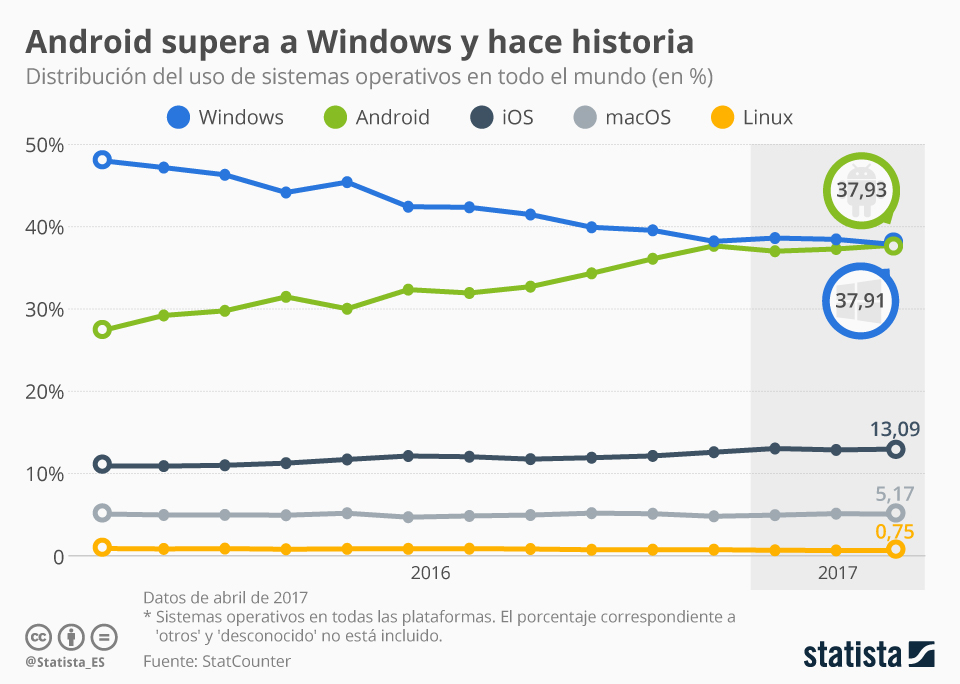
\includegraphics[scale=0.28]{Figures/SOMasUsado}
\end{frame}

\section{Comandos Básicos de Shell (Terminal)}
\begin{frame}
\begin{center}
\Huge{\textcolor{blue}{Comandos Básicos de Shell (Terminal)}} \\ \vspace{0.5cm}

\includegraphics[scale=0.4]{Figures/terminal}
\end{center}
\end{frame}

\begin{frame}
\begin{center}

\includegraphics[scale=0.2]{Figures/terminal}
\end{center}
\begin{itemize}
\item<2-|alert@2> \textbf{man:} Desplega el manual de comandos y programas.
\item<3-|alert@3> \textbf{ls:} Lista el contenido de un directorio.
\item<4-|alert@4> \textbf{pwd:} Muestra la ubicación actual.
\item<5-|alert@5> \textbf{more:} Permite ver el contenido de un archivo.
\item<6-|alert@6> \textbf{more:} Le da formato a la salida de un comando para visualizarlo por páginas.
\item<7-|alert@7> \textbf{less:} Igual que more, pero más pontente.
\item<8-|alert@8> \textbf{cd:} Cambia el directorio corriente (Change Directory) en que nos encontramos posicionados.
\item<9-|alert@9> \textbf{mkdir:} Crea entradas de directorios.
\item<10-|alert@10> \textbf{rmdir:} Elimina entradas de directorios vacíos.
\item<11-|alert@11> \textbf{rm:} Elimina archivos o directorios.
\end{itemize}
\end{frame}

\begin{frame}
\begin{center}

\includegraphics[scale=0.2]{Figures/terminal}
\end{center}
\begin{itemize}
\item<1-|alert@1> \textbf{cp:} Copiar archivos o directorios.
\item<2-|alert@2> \textbf{mv:} Mueve archivos o directorios.
\item<3-|alert@3> \textbf{echo:} Crea archivo de texto con la información dada.
\item<4-|alert@4> \textbf{cat:} Permite ver un archivo de texto.
\item<5-|alert@5> \textbf{find:} Permite buscar archivos.
\item<6-|alert@6> \textbf{grep:} Busca texto en un archivo.
\item<7-|alert@7> \textbf{wget:} Descargar el contenido de una URL en la red.
\item<8-|alert@8> \textbf{ps:} listado de procesos en ejecución.
\item<9-|alert@9> \textbf{kill:} Terminar o detener un proceso.
\item<10-|alert@10> \textbf{sudo:} Te permite realizar tareas que requieren permisos administrativos o raíz.
\item<11-|alert@11> \textbf{apt:} Comando que permite gestionar paquetes y aplicaciones.
\item<12-|alert@12> \textbf{tar:} Permite comprimir y descomprimir archivos.
\item<13-|alert@13> \textbf{exit:} Cierra la shell actual
\end{itemize}
\end{frame}

{\1
\begin{frame}[plain,noframenumbering]
  \finalpage{“¡El alcohol! La causa y solución de todos los problemas de la vida”, Homero Simpson  }
\end{frame}}

\end{document}